% !Mode:: "TeX:UTF-8"
%!TEX program  = xelatex

\documentclass[bwprint]{gmcmthesis}
\usepackage[framemethod=TikZ]{mdframed}
\title{全国研究生数学建模竞赛论文标题}
\baominghao{4321} %参赛队号
\schoolname{南京理工大学}%学校名称
\membera{周玉洁} %队员A
\memberb{刘婷婷} %队员B
\memberc{李宇轩} %队员C
\begin{document}

 %生成标题
 \maketitle

 %填写摘要
\begin{abstract}
本模板是为全国研究生数学建模竞赛编写的 \LaTeX{} 模板, 旨在让大家专注于
论文的内容写作, 而不用花费过多精力在格式的定制和调整上. 本手册是相应的参考, 其
中提供了一些环境和命令可以让模板的使用更为方便. 同时需要注意, 使用者需要有一
定的 \LaTeX{} 的使用经验, 至少要会使用 ctex 宏包的一些功能, 比如调节字距或修改字体
大小等等.
\end{abstract}

\begin{mdframed} [%
	roundcorner=5pt,
	linecolor=gray!50,
	outerlinewidth=0.5pt,
	middlelinewidth=0.3pt, backgroundcolor=gray!2,
innertopmargin=\topskip, frametitle={2020年格式变化说明},
frametitlefont= \bfseries,frametitlerule=true,frametitlealignment =\raggedright\noindent,
frametitlerulewidth=.5pt, frametitlebackgroundcolor=gray!2,]
今年的格式变化如下:
\begin{enumerate}
\item 论文第一页为标识替换。

\end{enumerate}

\end{mdframed}

\keywords{模板\quad  \LaTeX{}\quad   数学建模}

\pagestyle{plain}

%目录 不推荐加
%\tableofcontents
\newpage

\section{问题重述}

\subsection{引言}

创意平板折叠桌注重于表达木制品的优雅和设计师所想要强调的自动化与功能性。为了增大有效使用面积。设计师以长方形木板的宽为直径截取了一个圆形作为桌面,又将木板剩余的面积切割成了若干个长短不一的木条,每根木条的长度为平板宽到圆上一点的距离,分别用两根钢筋贯穿两侧的木条,使用者只需提起木板的两侧,便可以在重力的作用下达到自动升起的效果,相互对称的木条宛如下垂的桌布,精密的制作工艺配以质朴的木材,让这件工艺品看起来就像是工业革命时期的机器。

\subsection{问题的提出}

\subsubsection{问题一}

围绕创意平板折叠桌的动态变化过程、设计加工参数,本文依次提出如下问题:

(1)给定长方形平板尺寸 ($120 cm \times 50 cm \times 3 cm$),每根木条宽度(2.5 cm),连接桌腿木条的钢筋的位置,折叠后桌子的高度(53 cm)。要求建立模型描述此折叠桌的动态变化过程,并在此基础上给出此折叠桌的设计加工参数和桌脚边缘线的数学描述。



(2)折叠桌的设计应做到产品稳固性好、加工方便、用材最少。对于任意给定的折叠桌高度和圆形桌面直径的设计要求,讨论长方形平板材料和折叠桌的最优设计加工参数,例如,平板尺寸、钢筋位置、开槽长度等。对于桌高70 cm,桌面直径80 cm的情形,确定最优设计加工参数。


(3)给出软件设计的数学模型,可以根据客户任意设定的折叠桌高度、桌面边缘线的形状大小和桌脚边缘线的大致形状,给出所需平板材料的形状尺寸和切实可行的最优设计加工参数,使得生产的折叠桌尽可能接近客户所期望的形状,并根据所建立的模型给出几个设计的创意平板折叠桌。要求给出相应的设计加工参数,画出至少8张动态变化过程的示意图。

\section{模型的假设}

\begin{itemize}
\item 忽略实际加工误差对设计的影响;
\item 木条与圆桌面之间的交接处缝隙较小,可忽略;
\item 钢筋强度足够大,不弯曲;
\item 假设地面平整。
\end{itemize}

\section{符号说明}

\begin{tabular}{cc}
 \hline

 \makebox[0.4\textwidth][c]{符号}	&  \makebox[0.5\textwidth][c]{意义} \\ \hline
 D	    & 木条宽度(cm) \\ \hline
 L	    & 木板长度(cm)  \\ \hline
 W	    & 木板宽度(cm)  \\ \hline
 N	    & 第n根木条  \\ \hline
 T	    & 木条根数  \\ \hline
 H	    & 桌子高度(cm)  \\ \hline
 R	    & 桌子半径(cm)  \\ \hline
 R	    & 桌子直径(cm)  \\ \hline
\end{tabular}

\section{问题分析}

\subsection{问题一分析}
题目要求建立模型描述折叠桌的动态变化图,由于在折叠时用力大小的不同,我们不能描述在某一时刻折叠桌的具体形态,但我们可以用每根木条的角度变化来描述折叠桌的动态变化。首先,我们知道折叠桌前后左右对称,我们可以运用几何知识求出四分之一木条的角度变化。最后,根据初始时刻和最终形态两种状态求出桌腿木条开槽的长度。



\subsection{问题二分析}
题目要求从折叠桌的稳固性好、加工方便、用材最少三个角度,确定设计加工参数。我们可以从应力、支撑面积考虑稳固性,从开槽长度考虑加工方便,从木板长度考虑用材最少。而它们之间又是相互制约,我们需要确定最优设计加工参数,可以建立非线性规划模型,用lingo软件来求解最优设计加工参数(平板尺寸、钢筋位置、开槽长度等),这里以合力的方向(斜向上)与最长木条(桌腿)的夹角方向最小为目标函数,以木条所承受应力小于木条的许用应力、支撑面积大于桌面面积、木条的开槽长度小于木条本身长为约束条件。
\begin{figure}[!h]
\centering
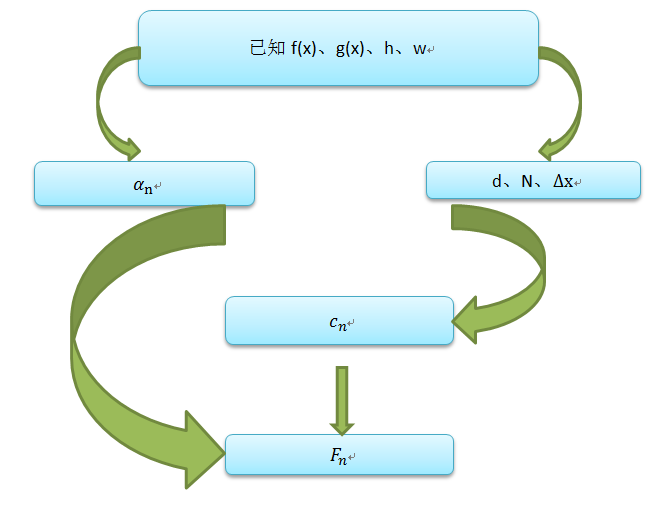
\includegraphics[width=.7\textwidth]{1.png}
\caption{问题三流程图}
\end{figure}
\subsection{问题三分析}
题目要求制作软件的意思就是客户给定折叠桌高度、桌面边缘线的形状大小和桌脚边缘线的大致形状,将这些信息输入程序就得到客户想要的桌子。我们在求解最优设计加工参数时,自行给定桌面边缘线形状(椭圆、相交圆等),桌脚边缘线形状,折叠桌高度,应用第二问的非线性规划模型,用MATLAB软件绘制折叠桌截面图,得到自己设计的创意平板折叠桌。

\newpage

\begin{thebibliography}{9}%宽度9
 \bibitem{bib:one} ....
 \bibitem{bib:two} ....
\end{thebibliography}   %参考文献

\newpage

\appendix
\section{源程序}
\begin{lstlisting}[language=Matlab]%设置不同语言即可。
kk=2;[mdd,ndd]=size(dd);
while ~isempty(V)
[tmpd,j]=min(W(i,V));tmpj=V(j);
for k=2:ndd
[tmp1,jj]=min(dd(1,k)+W(dd(2,k),V));
tmp2=V(jj);tt(k-1,:)=[tmp1,tmp2,jj];
end
tmp=[tmpd,tmpj,j;tt];[tmp3,tmp4]=min(tmp(:,1));
if tmp3==tmpd, ss(1:2,kk)=[i;tmp(tmp4,2)];
else,tmp5=find(ss(:,tmp4)~=0);tmp6=length(tmp5);
if dd(2,tmp4)==ss(tmp6,tmp4)
ss(1:tmp6+1,kk)=[ss(tmp5,tmp4);tmp(tmp4,2)];
else, ss(1:3,kk)=[i;dd(2,tmp4);tmp(tmp4,2)];
end;end
dd=[dd,[tmp3;tmp(tmp4,2)]];V(tmp(tmp4,3))=[];
[mdd,ndd]=size(dd);kk=kk+1;
end; S=ss; D=dd(1,:);
\end{lstlisting}     %附录

\end{document} 